\documentclass[class=report, crop=false, 12pt,a4paper, tikz, border=4mm]{standalone}
\usepackage{enumitem}
\usepackage{float}
\usepackage{amsmath}
\usepackage{amssymb}
\usepackage[normalem]{ulem}
\usepackage{graphicx}
\usepackage{siunitx}
\usepackage{tikz}
\usetikzlibrary{positioning, fit, calc}   
\tikzset{block/.style={draw, thick, text width=3cm ,minimum height=1.3cm, align=center},   
line/.style={-latex}     
}
\begin{document}
\section{Strain gauges}
\subsection{Strain}
The changes in the value of a dimension of a body divided by the original value of the dimension is the relative change in the dimensions. 
\begin{figure}[H]
  \centering
  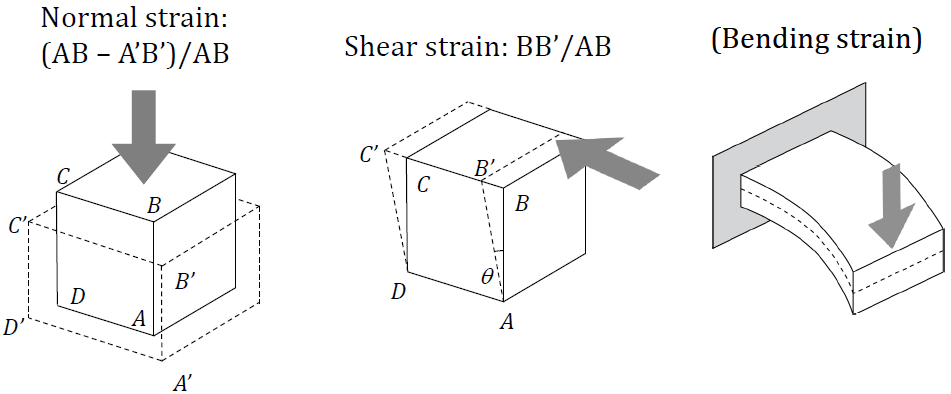
\includegraphics[width = 0.8 \textwidth]{../img/diagram8.png}
\end{figure}
Information about strain is required in many engineering situations: an aircraft in flight, support pillars and spans of bridges, etc.
\subsection{Stress}
Density of the reactive (internal) forces distributed throughout the body (force per unit area), in response to external force. Types of stress:
\begin{itemize}
  \item Tensile/compressive stress
  \item Shear stress
  \item Bending stress
\end{itemize}
Elastic modulus:
\begin{equation}
  E = \frac{\textrm{stress}}{\textrm{strain}}
\end{equation}
\begin{itemize}
  \item Young's modulus - normal strain (and if relationship is linear)
  \item Shear modulus - shear strain
  \item Bulk modulus - volumetric strain
\end{itemize}
\subsection{Strain gauges}
A device which experiences a change of electric resistance when it is strained. A strain gauge is combined with other electrical components to obtain an electric voltage or current representing tensile, compressive or bending strain, together wit the means of displaying or recording its value. The total resistance of a block of conducting material of uniform cross section $A$ and length $l$:
\begin{equation}
  R = \rho \frac{l}{A}
  \label{resistance}
\end{equation}
Where $\rho$ is resistivity with units \si{\ohm \meter}.
\begin{figure}[H]
  \centering
  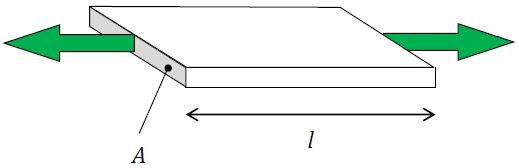
\includegraphics[width = 0.8 \textwidth]{../img/diagram9.png}
  \caption{When the block is subjected to a tensile stress, its length will increase and cross-sectional area will decrease, both of which cause the resistance to increase according to equation (\ref{resistance})}
\end{figure}
The resistivity of the material will also change because of the \textbf{piezo-resistive effect} (increase with tension and decrease with compression). The resistance of the block can thus be written as:
\begin{equation}
  R' = (\rho + \delta \rho) \frac{l + \delta l}{A - \delta A}
\end{equation}
Note: compressive stress will result in a decrease in total resistance.
\subsection{Simple wire strain gauge}
A long fine wire is folded to fit in a small area and then mounted on a flexible backing sheet, usually paper. When \textbf{firmly stuck} to the surface of a much more rigid body, any deformation of this body will cause an identical fractional change of the strain gauge wire. The change of resistance for any strain along the active axis will be much greater than for an equal strain occurring along the passive axis.
\begin{figure}[H]
  \centering
  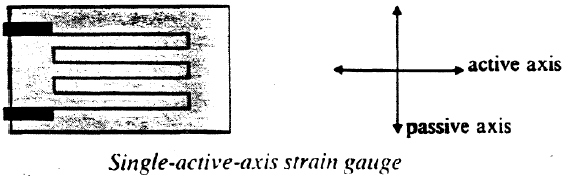
\includegraphics[width = 0.8 \textwidth]{../img/diagram10.png}
\end{figure}
\subsection{Gauge factor}
Defined as the fractional change of resistance of the gauge, divided by the fractional change in the length of the gauge along the active axis:
\begin{equation}
  G = \frac{\frac{\Delta R}{R}}{\frac{\Delta l}{l}}
\end{equation}
Since $\frac{\Delta l}{l}$ is the strain $e$ in the body to which the gauge is fixed, this can be rewritten as:
\begin{equation}
  \frac{\Delta R}{R} = eG
\end{equation}
Most gauges have a $G$ between \textbf{1.8 to 2.2}, depending on the gauge material and the magnitude of the piezo-resistive effect.
\subsection{Foil strain gauge}
Most modern strain gauges are formed by rolling out a thin foil of the resistive material and then cutting away parts of the foil by a photo-etching process, to create the required grid pattern.
\begin{itemize}
  \item Usually supplied with think backing paper as electrical insulation
  \item Adhesive layer for the fixation to the specimen should be creep-free and allow heat dissipation
\end{itemize}
Advantages over simple wire strain gauges:
\begin{itemize}
  \item Larger surface area results in a larger area of adhesion
  \item Accurate reproducibility due to photo-etching technique
  \item Small dimensions mean they are good for localised strain, fit well to curvature
\end{itemize}
\subsection{How can we measure strain}
\begin{figure}[H]
  \centering
  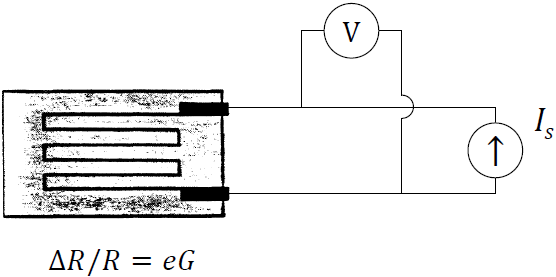
\includegraphics[width = 0.8 \textwidth]{../img/diagram11.png}
  \caption{Is this good enough?}
\end{figure}
Typically $e = 10^{-3}, \ G = 2.1, \ R = 120 \si{\ohm}, \ I_S < 50 \si{\milli \ampere}$.
\begin{gather}
  V = 6 \si{\volt}, \ \Delta R = 0.252 \si{\ohm}\\
  \Delta V = 0.013 \si{\volt}
\end{gather}
The fractional change of the voltage is too small to detect comparing to the 'baseline' voltage $(=RI_S)$.
\section{Wheatstone bridge}
Used to convert the change of resistance in the strain gauge into an electrical signal which could be used to indicate the value of strain. With this, \textbf{zero strain $\leftrightarrow$ zero output voltage}.
\begin{figure}[H]
  \centering
  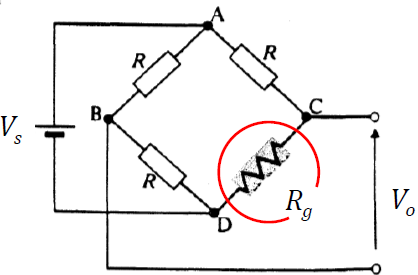
\includegraphics[width = 0.6 \textwidth]{../img/diagram12.png}
\end{figure}
Here, 
\begin{equation}
  V_C - V_D = \frac{V_S R_G}{R + R_G}
\end{equation}
and then,
\begin{equation}
  V_0 = V_C - V_B = \left( V_D + \frac{V_S R_G}{R + R_G} \right) - \left( V_D + \frac{V_S}{2} \right) = \frac{V_S R_G}{R + R_G} - \frac{V_S}{2}
\end{equation}
$R$ is chosen to have the same value as the unstrained gauge, i.e. $R = R_G$ when zero strain $\rightarrow V_0 = 0$ when zero strain. When the gauge is strained, $R_G = R + r$ and the output voltage is
\begin{equation}
  V_0 = V_S \frac{R + r}{2R + r} - \frac{V_S}{2} = V_S \frac{r}{2(2R +r)}
\end{equation}
Now using the gauge factor, $\frac{r}{R} = eG$ and the equation can be rewritten: 
\begin{equation}
  V_0 = V_S \frac{ReG}{2(2R + ReG)} = V_S\frac{eG}{2(2+eG)} \approx \frac{1}{4} V_S eG
\end{equation}
Because typically $eG < 0.02 << 2$

Sensitivity:
\begin{equation}
  \frac{V_0}{e} = \frac{1}{4} V_S G
\end{equation}
\subsection{Temperature compensation}
The output voltage from the strain gauge and the bridge also depends on the temperature. Changes in temperature will cause changes in:
\begin{itemize}
  \item Dimensions of the specimen and hence the gauge due to thermal expansion
  \item Dimensions of the gauge itself (particularly thickness)
  \item Resistivity of the gauge material
\end{itemize}
Compensated with a dummy gauge:
\begin{figure}[H]
  \centering
  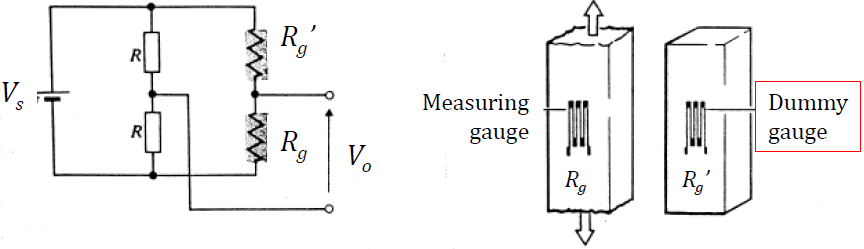
\includegraphics[width = 0.8 \textwidth]{../img/diagram13.png}
\end{figure}
The output voltage of the bridge is: 
\begin{equation}
  V_0 = V_S \frac{R_G}{R_G + R_G'} - \frac{V_S}{2}
\end{equation}
Substituting for $R_G$ and $R_G'$, we have:
\begin{gather}
  V_0 = V_S \frac{R(1+x){1+y}}{R(1+x){1+y} + R(1+y)} - \frac{V_S}{2}\\
  \frac{V_0}{V_S} = \frac{R(1+x){1+y}}{R(1+x){1+y} + R(1+y)} - \frac{1}{2} \leftarrow \textrm{no influence by y}
\end{gather}
However, for this you must find the specimen of the same material and keep them under the same temperature - are these easy enough? The dummy gauge could be placed on the same member as the measuring gauge with its active axis in the direction normal to that of the strain.
\end{document}